\documentclass[conference]{IEEEtran}

\usepackage{cite}
\usepackage{graphicx}
\usepackage{amsmath,amssymb}
\usepackage{textcomp}
\usepackage{booktabs}
\usepackage[caption=false,font=footnotesize]{subfig}
\usepackage{url}

\newcommand{\hzo}{Hf$_{0.5}$Zr$_{0.5}$O$_2$}
\newcommand{\xir}{\xi_{r}}
\newcommand{\CMW}{\mathrm{CMW}}
\newcommand{\fc}{f_{c}}
\newcommand{\Ecross}{E_{\mathrm{cross}}}
\newcommand{\uCcm}{\,$\mu$C/cm$^{2}$}
\newcommand{\MVcm}{\,MV/cm}

\begin{document}

\title{Maxwell--Wagner Relaxation Limits Zero-Bias Capacitive Memory Window Readout in Ferroelectric \hzo{} Capacitors}

\author{\IEEEauthorblockN{Apu Das and Sourav De}
\IEEEauthorblockA{College of Semiconductor Research, National Tsing Hua University, Hsinchu 300044, Taiwan\\
Email: apudas@nthu.edu.tw, sourav.de@mx.nthu.edu.tw}}

\maketitle

\begin{abstract}
The zero-bias capacitive memory window (CMW) enables non-destructive readout in ferroelectric capacitors, but its practical bandwidth is not set by polarization alone. We compare two \hzo{} capacitor stacks by frequency-resolved $C$--$V$ spectroscopy from 1~kHz to 4~MHz together with PUND and switching-current measurements at 300~K and 10~K. The CMW of TaN/\hzo{}/TiN relaxes as a single Debye process with $\fc = 179$~kHz, while a WO$_x$-bearing stack with nearly the same low-frequency dielectric ceiling relaxes at $\fc = 1.4$~kHz. At 10~K the capacitive read window falls below 1~kHz even though polarization switching persists. The data support an interface-limited Maxwell--Wagner mechanism: polarization stores the bit, but interfacial conductivity sets whether and how fast the states remain capacitively distinguishable.
\end{abstract}

\begin{IEEEkeywords}
Ferroelectric capacitor, hafnium zirconium oxide, capacitive memory window, non-destructive readout, Maxwell--Wagner relaxation.
\end{IEEEkeywords}

\section{Introduction}
Ferroelectricity in doped HfO$_2$ and especially in \hzo{} has reopened the path to scalable ferroelectric memory compatible with CMOS and BEOL processing~\cite{boscke2011,muller2012,schroeder2022}. In a conventional ferroelectric capacitor, however, reading the stored state is destructive because the switched charge $2P_r$ must be sensed by driving the device through its coercive field. A capacitive read avoids that penalty. The two remanent polarization states occupy different small-signal permittivity branches, so a sub-coercive capacitance measurement can distinguish the stored bit without forcing a rewrite~\cite{luo2020}. That possibility is attractive for read-dominated memory operation and for analog or in-memory computing schemes that repeatedly interrogate the same stored state.

Prior work established that a capacitive memory window can be opened and enlarged by interface engineering, and that non-destructive readout can be demonstrated in BEOL-compatible ferroelectric capacitors and array-relevant circuits~\cite{mukherjee2023iedm,lee2025aem}. What those reports do not resolve is the physics that governs the window itself. A large remanent polarization is necessary to define two stored states, but it is not sufficient to guarantee a useful zero-bias CMW: in an ideally symmetric stack, the two $C$--$V$ branches would still intersect at zero bias. The practical questions are therefore sharper than simply asking whether ferroelectricity is present. What determines the usable read bandwidth? Why does the zero-bias window vary between stacks? And will the same readout survive across temperature?

The full TMAT paper addresses those questions by testing two competing pictures. In a ferroelectric-limited picture, the CMW should follow the intrinsic dielectric and switching dynamics of the \hzo{} layer and therefore persist on the ferroelectric timescale. In an interface-limited picture, the window should relax with the impedance of the interfacial region and should change strongly with stack design and temperature. This conference version retains the decisive evidence for the latter view. It develops the argument around one statement: polarization stores the bit, but the interface sets whether and how fast the two states remain capacitively distinguishable.


\section{Experimental Methods}
Two metal--ferroelectric--metal capacitors were compared. Stack~A was TaN/\hzo{}(10~nm)/TiN on Si. Stack~B was TiN/PE-TiN/\hzo{}/WO$_x$/W on Si, where the deliberate WO$_x$ layer modifies the bottom interface and provides a second stack with a different interfacial impedance. Grazing-incidence XRD was used to confirm crystallization of the ferroelectric films, while the electrical study focused on the relation between the two remanent branches of the small-signal dielectric response.

Frequency-resolved $C$--$V$ measurements were performed in parallel $C_p$--$R_p$ mode with a 50~mV rms signal at 61 logarithmically spaced frequencies from 1~kHz to 4~MHz. The dc bias was swept $-2 \rightarrow +2 \rightarrow -2$~V so that the two polarization branches were collected under identical conditions. For each frequency, the zero-bias capacitive memory window was obtained from the branch separation,
\begin{equation}
\CMW_\xi(f)=\xi_\downarrow(0,f)-\xi_\uparrow(0,f),
\label{eq:cmw_short}
\end{equation}
where $\xi_\uparrow$ and $\xi_\downarrow$ denote the branches reached after opposite preset states. The crossing field $\Ecross$ was taken from the bias at which the two branches became capacitively indistinguishable.

To test whether changes in the window simply mirrored changes in polarization, the capacitive data were paired with PUND and switching-current measurements. The same devices were measured at 300~K and 10~K so that the zero-bias readout and the switching response could be compared on the same temperature axis. High-frequency interpretation was limited to the range below the series-resistance-dominated region identified from the measured roll-off and standard dielectric-analysis practice~\cite{nicollian1982,schroder2006}.


\section{Results and Discussion}
The starting point is the contrast between the two stacks at low frequency. At 1~kHz, both devices show the butterfly-shaped permittivity characteristic of ferroelectric \hzo{}, and both reach a similar peak relative permittivity of about 62. Yet the zero-bias state separation is different: Stack~A gives $\CMW_\xi \approx 5.2$, whereas Stack~B gives only $\approx 2.3$ [Fig.~\ref{fig:cmw}]. This immediately suggests that the zero-bias read margin is not set only by the ferroelectric dielectric amplitude. As the measurement frequency increases, the branch separation collapses while a substantial background permittivity remains. The disappearing quantity is therefore the state discrimination itself, not the dielectric response as a whole.

The frequency dependence of that state discrimination is captured by a single-Debye form,
\begin{equation}
\CMW(f)=\frac{\CMW_0}{1+(f/\fc)^2},
\label{eq:debye_short}
\end{equation}
which directly isolates the relaxing part of the zero-bias window. Fits to Fig.~\ref{fig:debye} give $\CMW_0=5.38$ and $\fc=179$~kHz for Stack~A, corresponding to $\tau=0.90\,\mu$s, while Stack~B relaxes much more slowly with $\CMW_0=3.6$ and $\fc=1.4$~kHz ($\tau=114\,\mu$s). The full TMAT dataset shows that the differential loss and Cole--Cole representations return the same characteristic corner and do not require a distributed relaxation spectrum. That behavior is consistent with one dominant relaxation process rather than with a broad intrinsic ferroelectric response~\cite{jonscher1983,colecole1941}.

Temperature provides an independent discriminator. At 10~K, Stack~A still switches: $2P_r$ decreases from 33.1 to 20.3\uCcm{} and $E_c$ increases from 0.93 to 1.17\MVcm{}, but the device remains ferroelectric [Fig.~\ref{fig:cryo}]. The capacitive readout changes more severely. The zero-bias CMW falls from 5.2 to about 2.2 at 1~kHz and then drops to the noise floor above 1.1~kHz, implying $\fc \lesssim 1$~kHz at 10~K. Cooling therefore suppresses the capacitive-read bandwidth by more than two decades even though polarization reversal remains observable. That decoupling is difficult to reconcile with a read mechanism controlled only by the ferroelectric switching timescale.

The strongest argument comes from comparing the two stacks directly. Their low-frequency dielectric ceilings are nearly identical, so the ferroelectric layer presents essentially the same dielectric amplitude in both devices. Nevertheless, the relaxation times differ by $126\times$ [Table~\ref{tab:summary}], and the stack containing the deliberate WO$_x$ interface is the slower one. A compact Maxwell--Wagner description,
\begin{equation}
\tau \approx \frac{\varepsilon_i}{\sigma_i},
\label{eq:mw_short}
\end{equation}
assigns that timescale to the interfacial layer rather than to the ferroelectric bulk~\cite{alcala2023,kremer2003}. The extracted interfacial areal capacitances differ only modestly (2.95 versus 2.34~$\mu$F/cm$^2$), whereas the corresponding areal resistances differ by about $157\times$. In other words, the two stacks share nearly the same dielectric ceiling but not the same interface clock.

Taken together, the full plot set supports a simple reading rule for the reduced manuscript. The zero-bias CMW exists because polarization creates two stored states, but the rate at which those states remain capacitively distinguishable is controlled by interfacial charge relaxation. The metric reported at a single frequency is therefore not portable by itself. For conference presentation, the critical outputs are the low-frequency window, the fitted corner frequency, and the interface-sensitive comparison that shows why the same ferroelectric can yield very different NDRO read bandwidths.


\section{Conclusion}
The conference version reduces the manuscript to one governing result: zero-bias capacitive readout in ferroelectric \hzo{} capacitors is limited by an interfacial Maxwell--Wagner relaxation rather than by the ferroelectric's intrinsic switching timescale. The CMW collapses with frequency while a substantial dielectric response remains, its relaxation follows a single-Debye law, and cooling suppresses the read bandwidth far more strongly than switching itself. Because two stacks with nearly identical dielectric ceilings differ by more than two orders of magnitude in relaxation time, the usable NDRO read band is an interface property. Reported CMW values must therefore be tied to measurement frequency and stack design.

\bibliographystyle{IEEEtran}
\bibliography{1_mainbody/references}

\clearpage
\begin{figure}[!t]
\centering
\subfloat[]{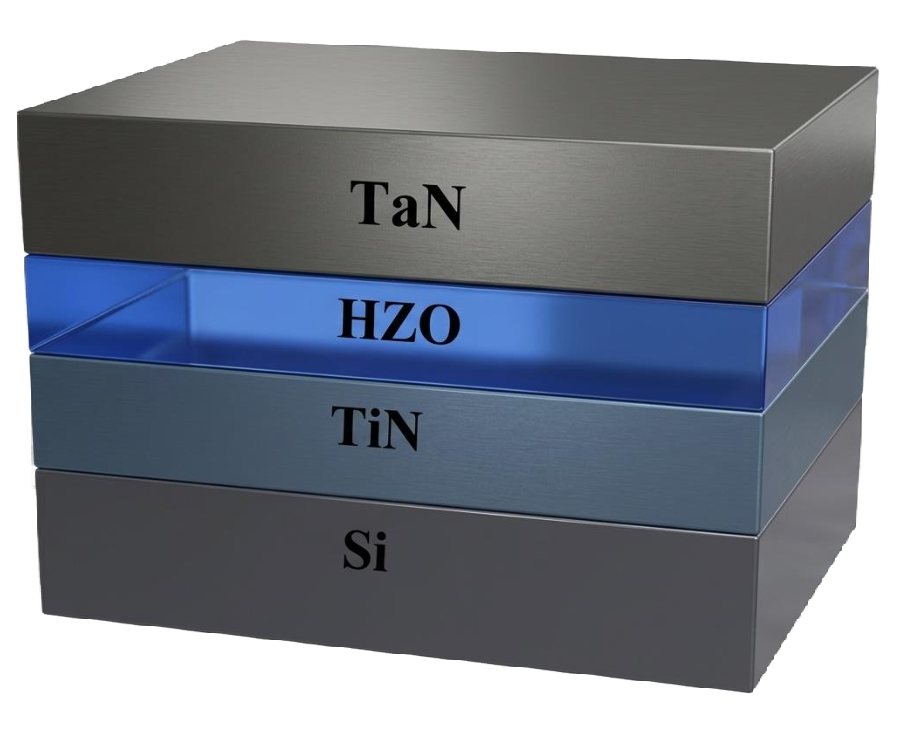
\includegraphics[width=0.47\columnwidth]{figures/fig 1a.pdf}\label{fig:stacks_a}}
\hfill
\subfloat[]{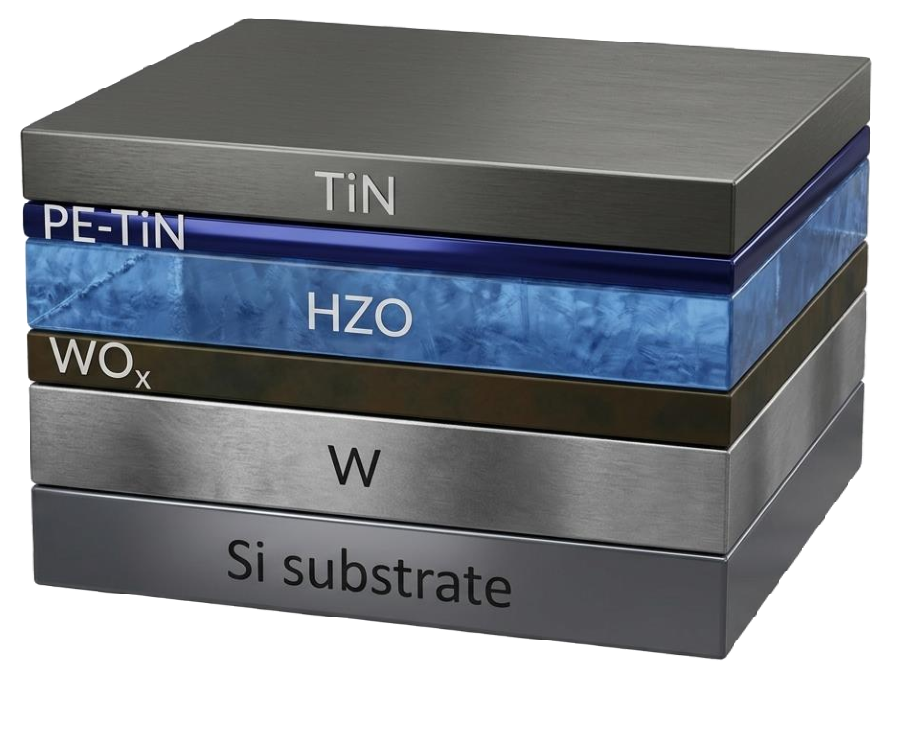
\includegraphics[width=0.47\columnwidth]{figures/fig 1b.pdf}\label{fig:stacks_b}}\\
\subfloat[]{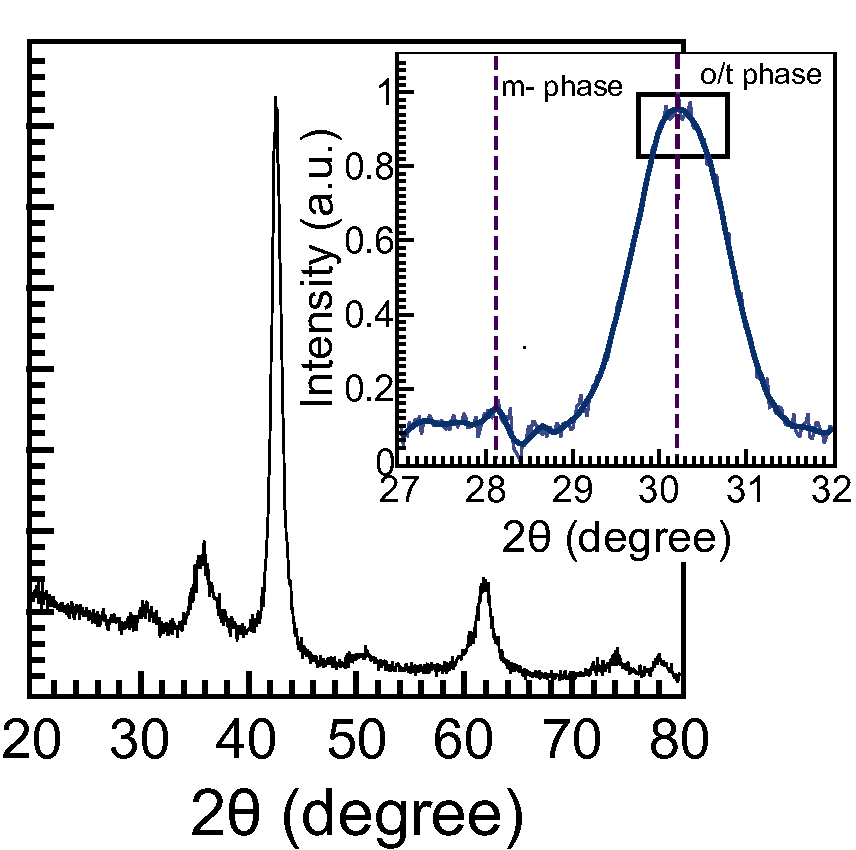
\includegraphics[width=0.47\columnwidth]{figures/1f_XRD Full.pdf}\label{fig:stacks_c}}
\hfill
\subfloat[]{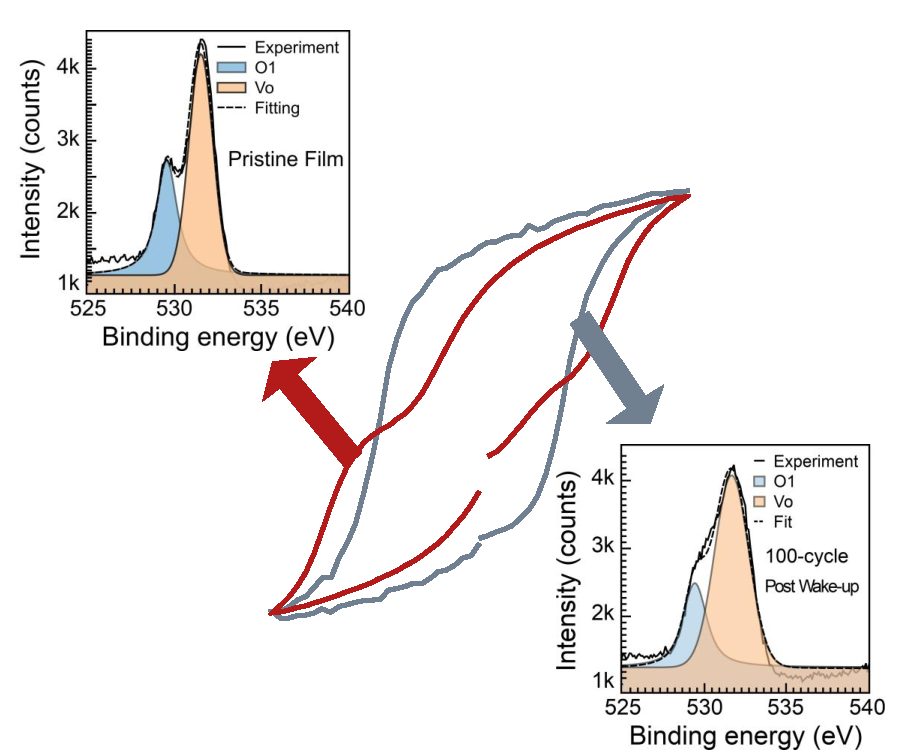
\includegraphics[width=0.47\columnwidth]{figures/fig 1d.pdf}\label{fig:stacks_d}}
\caption{Device and materials context. (a), (b) The compared capacitor stacks differ mainly in their electrode/interface design. (c) GIXRD confirms ferroelectric-phase formation in the \hzo{} films. (d) Polarization and interfacial-chemistry context from the source manuscript motivate the interface-focused interpretation used in this four-page version.}
\label{fig:stacks}
\end{figure}

\begin{figure}[!t]
\centering
\subfloat[]{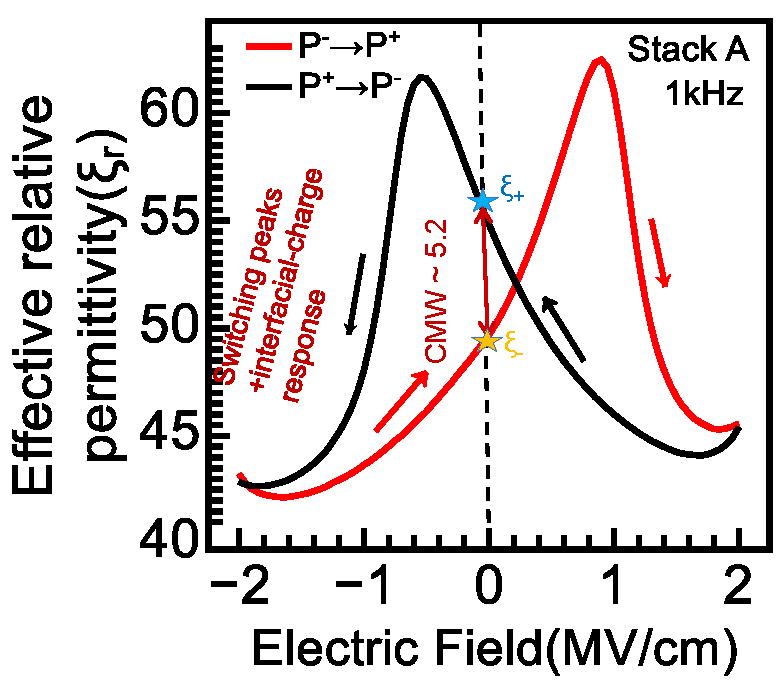
\includegraphics[width=0.47\columnwidth]{figures/fig 2a.pdf}\label{fig:cmw_a}}
\hfill
\subfloat[]{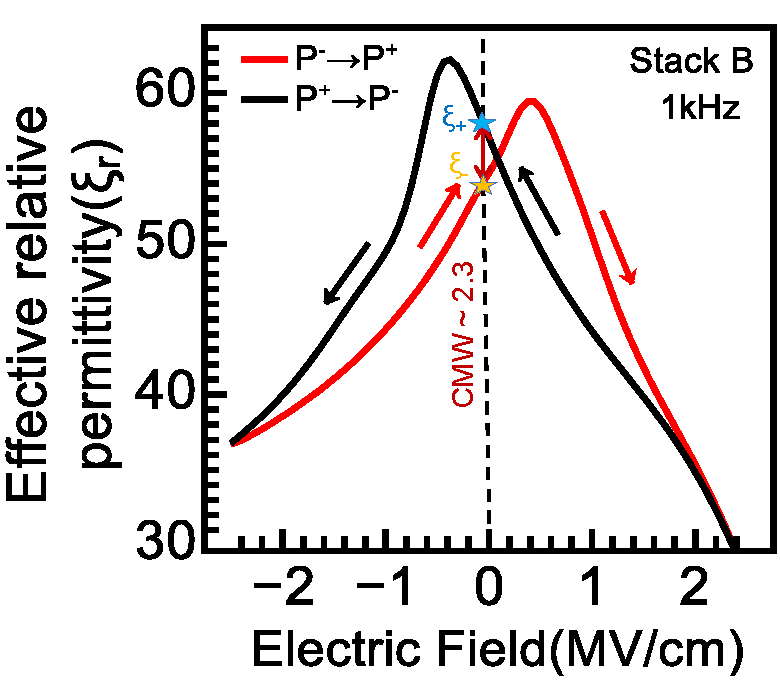
\includegraphics[width=0.47\columnwidth]{figures/fig 2b.pdf}\label{fig:cmw_b}}\\
\subfloat[]{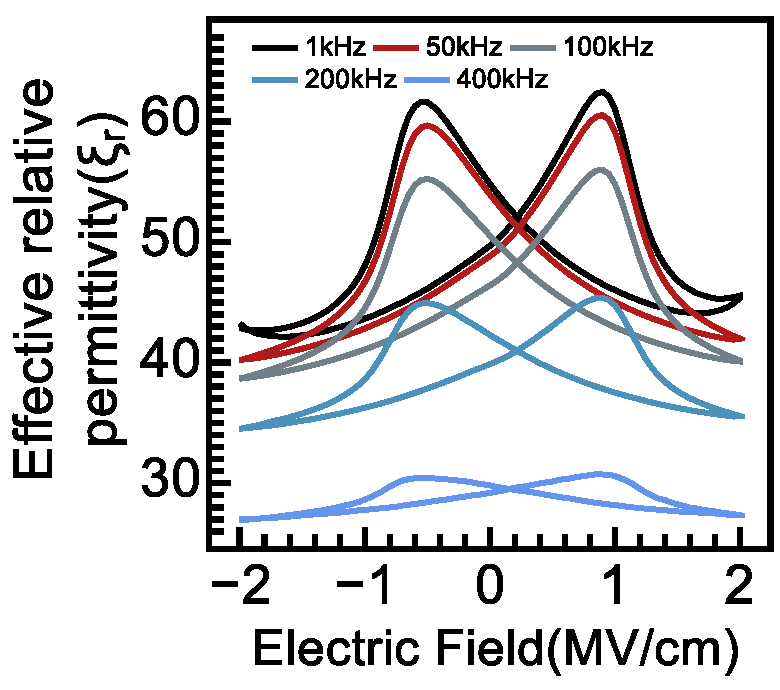
\includegraphics[width=0.47\columnwidth]{figures/fig 2c.pdf}\label{fig:cmw_c}}
\hfill
\subfloat[]{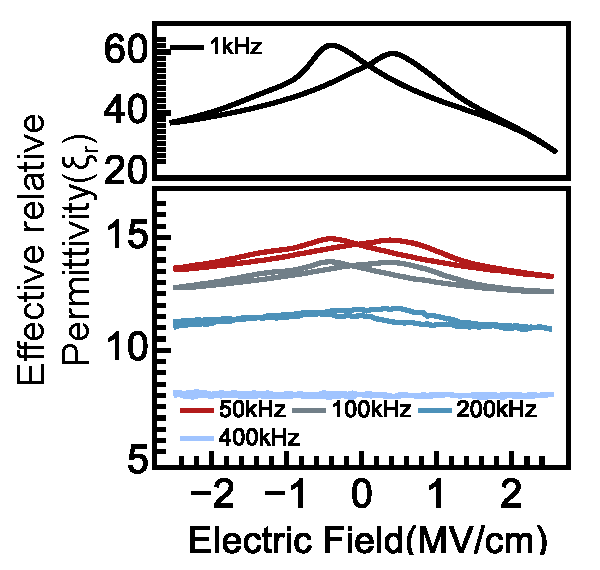
\includegraphics[width=0.47\columnwidth]{figures/fig 2d.pdf}\label{fig:cmw_d}}
\caption{Definition and collapse of the zero-bias CMW. Stack~A shows $\CMW_\xi \approx 5.2$ at 1~kHz, while Stack~B shows $\approx 2.3$ at a similar peak permittivity. With increasing frequency, the branch separation collapses while a substantial dielectric response remains, showing that the lost quantity is the state discrimination rather than the full capacitance.}
\label{fig:cmw}
\end{figure}

\begin{figure}[!t]
\centering
\subfloat[]{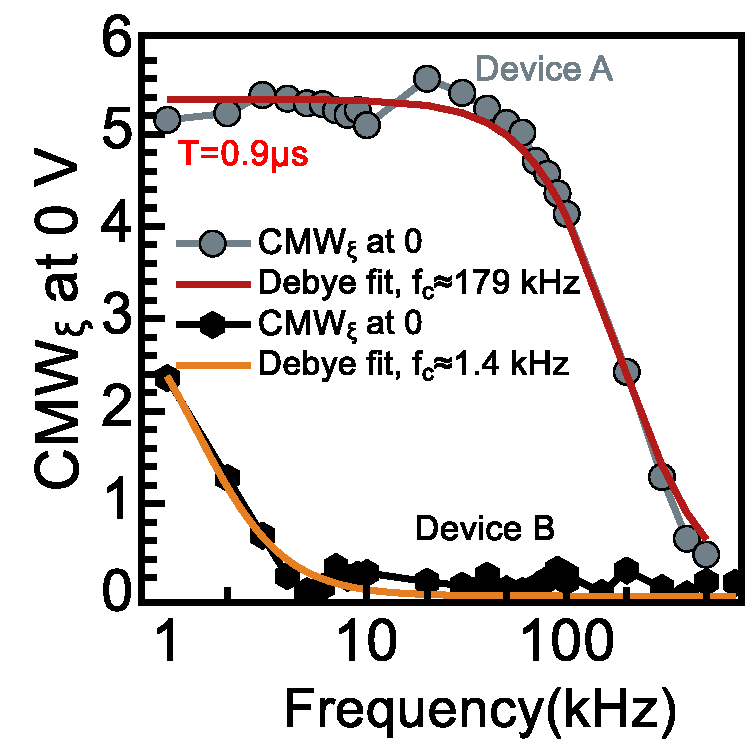
\includegraphics[width=0.31\columnwidth]{figures/fig 3a.pdf}\label{fig:debye_a}}
\hfill
\subfloat[]{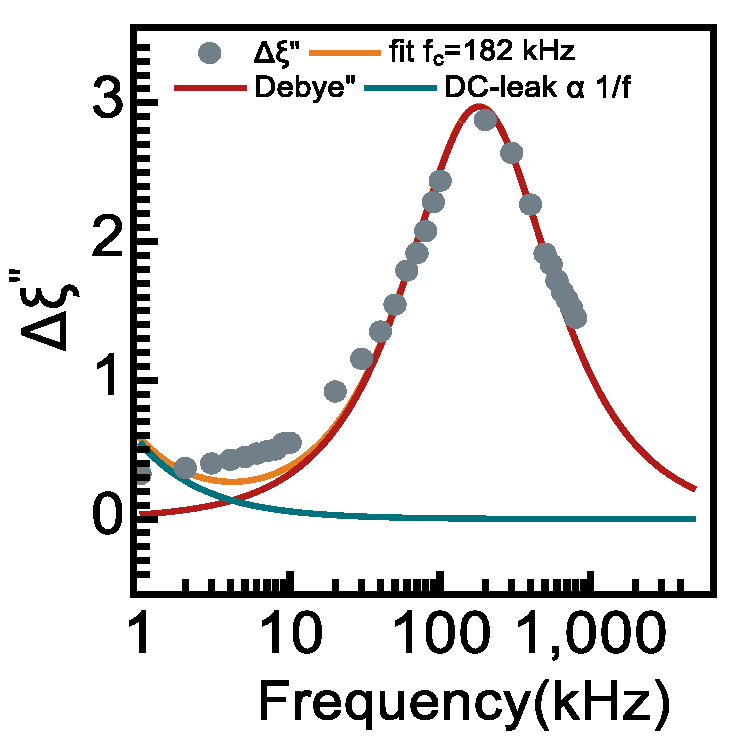
\includegraphics[width=0.31\columnwidth]{figures/fig 3b.pdf}\label{fig:debye_b}}
\hfill
\subfloat[]{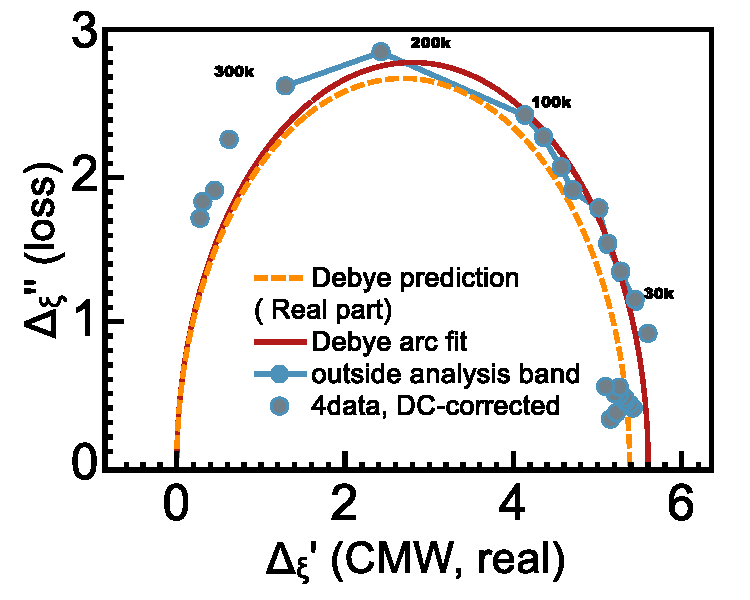
\includegraphics[width=0.31\columnwidth]{figures/fig 3c.pdf}\label{fig:debye_c}}
\caption{Single-process relaxation evidence. The CMW roll-off, differential loss, and Cole--Cole response are all consistent with a single-Debye relaxation, giving $\fc=179$~kHz for Stack~A and $\fc=1.4$~kHz for Stack~B.}
\label{fig:debye}
\end{figure}

\begin{figure}[!t]
\centering
\subfloat[]{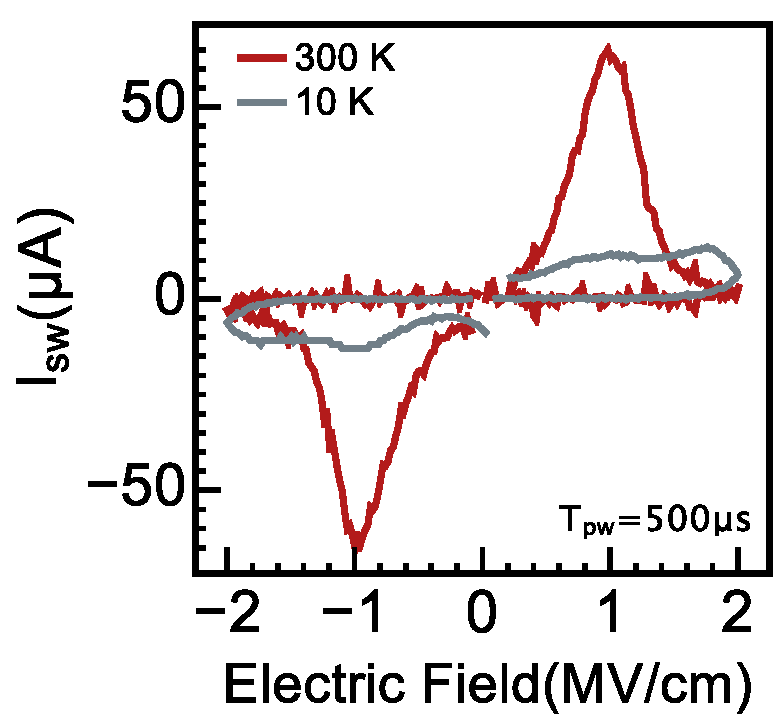
\includegraphics[width=0.47\columnwidth]{figures/fig 4a.pdf}\label{fig:cryo_a}}
\hfill
\subfloat[]{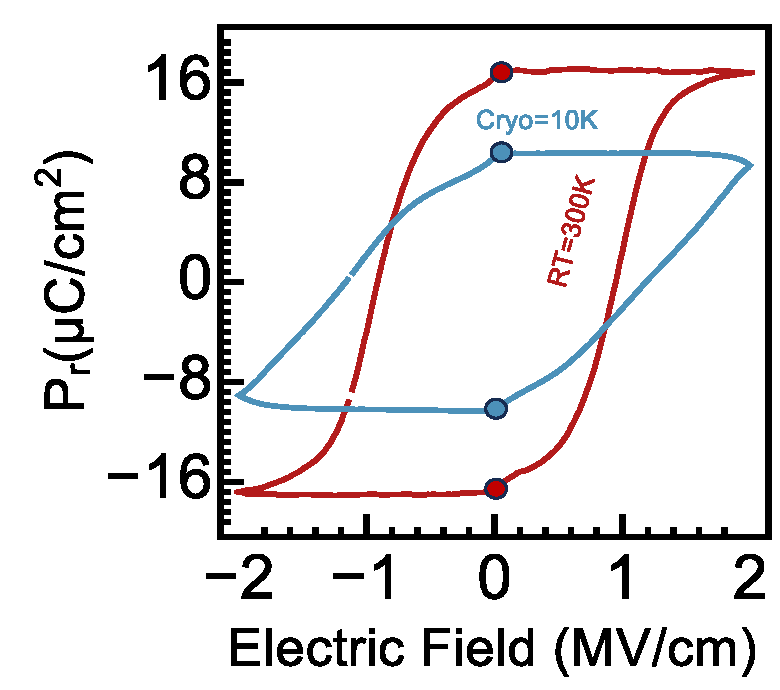
\includegraphics[width=0.47\columnwidth]{figures/fig 5b.pdf}\label{fig:cryo_b}}\\
\subfloat[]{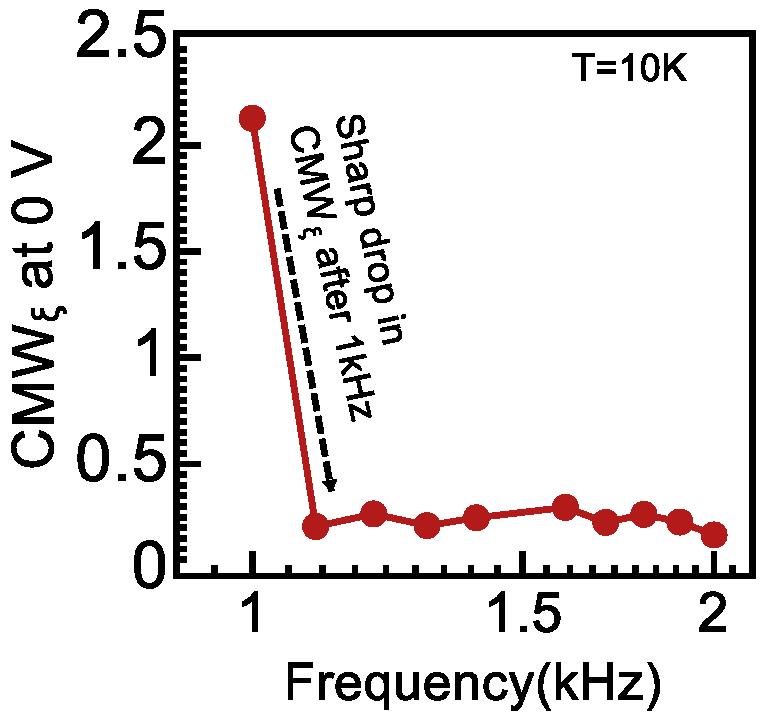
\includegraphics[width=0.47\columnwidth]{figures/fig 4d.pdf}\label{fig:cryo_c}}
\hfill
\subfloat[]{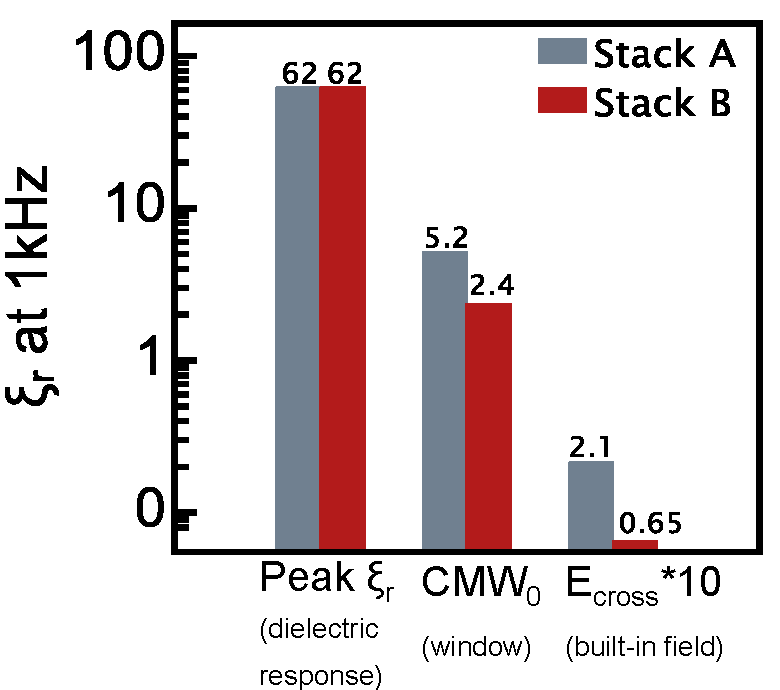
\includegraphics[width=0.47\columnwidth]{figures/figure3/fig 3e.pdf}\label{fig:cryo_d}}
\caption{Temperature and interface summary. At 10~K, switching persists but the zero-bias CMW bandwidth collapses below 1~kHz. The cross-stack summary shows nearly identical low-frequency dielectric ceilings together with large differences in CMW amplitude and clock speed, consistent with interface-controlled readout.}
\label{fig:cryo}
\end{figure}

\begin{table}[!t]
\renewcommand{\arraystretch}{1.08}
\caption{Key Parameters Retained for the 4-Page Version}
\label{tab:summary}
\centering
\scriptsize
\setlength{\tabcolsep}{3pt}
\begin{tabular}{@{}lcc@{}}
\toprule
Parameter & Stack A & Stack B \\
\midrule
Peak $\xir$ at 1 kHz & 62.5 & 62.2 \\
Ceiling $\xir(0)$ & $62.4\pm1.2$ & $62.7\pm0.9$ \\
CMW at 1 kHz & 5.2 & 2.4 \\
$\CMW_0$ (fit) & 5.38 & 3.6 \\
$\fc$ & 179 kHz & 1.4 kHz \\
$\tau$ & 0.90 $\mu$s & 114 $\mu$s \\
$\Ecross$ & 0.221 MV/cm & 0.081 MV/cm \\
$c_{IL}$ & 2.95 $\mu$F/cm$^2$ & 2.34 $\mu$F/cm$^2$ \\
$R_{IL}$ & 0.31 $\Omega\cdot$cm$^2$ & 48.8 $\Omega\cdot$cm$^2$ \\
\midrule
$2P_r$ at 300 K / 10 K & \multicolumn{2}{c}{33.1 / 20.3 $\mu$C/cm$^2$} \\
CMW at 300 K / 10 K & \multicolumn{2}{c}{5.2 / 2.2 (Stack~A)} \\
$\fc$ at 300 K / 10 K & \multicolumn{2}{c}{179 kHz / $\lesssim$1 kHz (Stack~A)} \\
\bottomrule
\end{tabular}
\end{table}


\end{document}
